\documentclass{article}

% Please use the following line and do not change the style file.
\usepackage{icml2021_author_response}

% Recommended, but optional, packages for figures and better typesetting:
\usepackage{microtype}
\usepackage{graphicx}
\usepackage{subfigure}
\usepackage{hyperref}       % hyperlinks
\usepackage{booktabs} % for professional tables
\usepackage{amsfonts}       % blackboard math symbols
\usepackage{nicefrac}       % compact symbols for 1/2, etc.
\usepackage{url}
\usepackage{lipsum}

\begin{document}
% Uncomment the following line if you prefer a single-column format
%\onecolumn

% Reviews in https://docs.google.com/document/d/1QU7Wp6Mdy2oXFt71Etj0X6PbwRFFPS7V5ghuOlVvtSE/edit?usp=sharing

\section{General Response}
We thank the reviewers for their thoughtful feedback. We propose a general kernel method to speed up inference in structured prediction and demonstrate its efficacy in both HMMs and PCFGs. Reviewers noted that the experimental evaluation could be improved by increasing the number of HMM states and incorporating speed comparisons. 

%In response, we will make the following changes, which show that LHMMs are able to achieve similar performance to softmax HMMs in a fraction of the time.

%\vspace{-0.2cm}
\subsection{Larger State Sizes / Feature Ratios (R1, R5)}
We compare perplexities between softmax HMMs and LHMMs (our model) across larger state spaces, up to $2^{14}$ (16k) states (expanded from 4k states).
In Figure~\ref{fig:ppl},
we find that with a 4:1 state-to-feature ratio LHMMs are able to achieve the same perplexity as softmax HMMs with the same number of states, while an 8:1 ratio underperforms softmax HMMs.
\begin{figure}[!htp]
  \centering
    \vspace*{-0.3cm}
  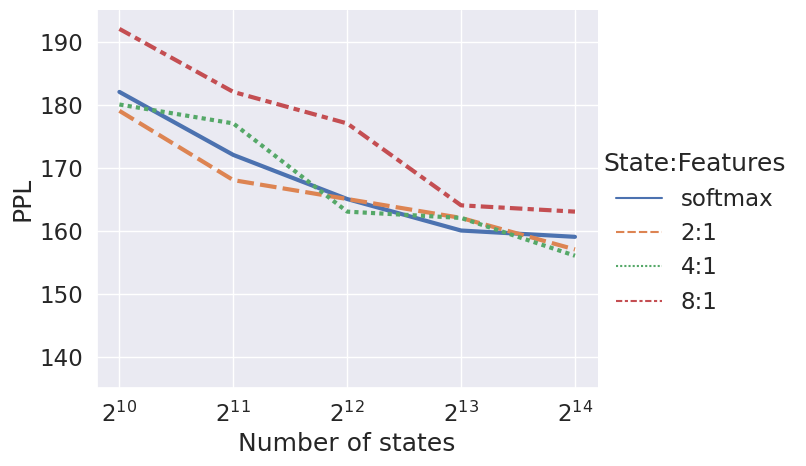
\includegraphics[width=0.46\textwidth]{imgs/hmm/lhmm-states-features.png}
  \vspace*{-0.5cm}
  \caption{\label{fig:ppl}
  Softmax HMMs and LHMMs at different state sizes.
  }
  \vspace{-0.4cm}
\end{figure}
However, we are able to scale the state-to-feature ratio with state dropout, a technique the reviewers point out from VL-HMM (Chiu and Rush, 2020). In Figure~\ref{fig:dropout}, we see that LHMMs achieve similar performance to the baseline at $2^{14}$ states with an 8:1 state-to-feature ratio.
\begin{figure}[!htp]
  \centering
  \vspace*{-0.3cm}
  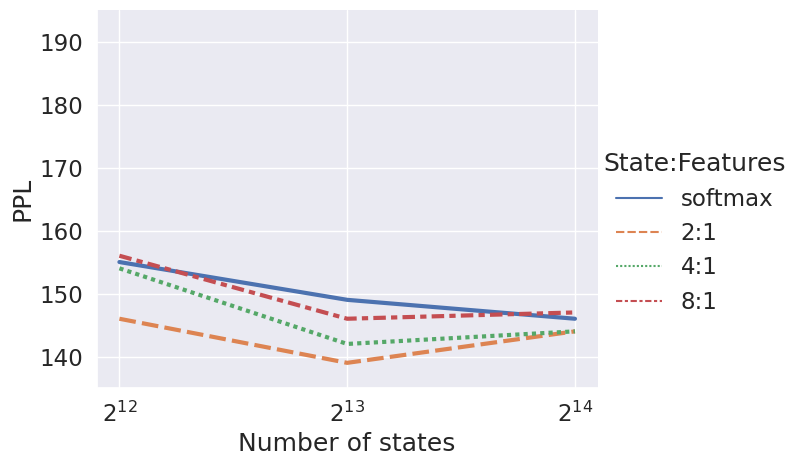
\includegraphics[width=0.46\textwidth]{imgs/hmm/lhmm-states-features-dropout.png}
  \vspace*{-0.5cm}
  \caption{\label{fig:dropout}
  Softmax HMMs and LHMMs with 0.1 state dropout.
  %Perplexities are noisy due to local optima in EM,
  %the LHMM model with $2^{14}$ overfit as we kept the dropout rate constant.
}
\vspace{-0.6cm}
\end{figure}

%\vspace{-0.2cm}
\subsection{Speed Comparisons (R1, R3, R5)}
%We will also include the speed comparisons for large LHMMs and softmax HMMs on GPUs. 
In theory, LHMMs should get a speedup of 2x for a 4:1 state-to-feature ratio, and 4x for an 8:1 ratio due to reducing the quadratic term but adding an additional linear term. Experimentally, we find that in Figure~\ref{fig:speed} our implementation achieves this goal at the same accuracy. 

%without and with state dropout respectively.
\begin{figure}[!htp]
  \centering
  \vspace*{-0.3cm}
  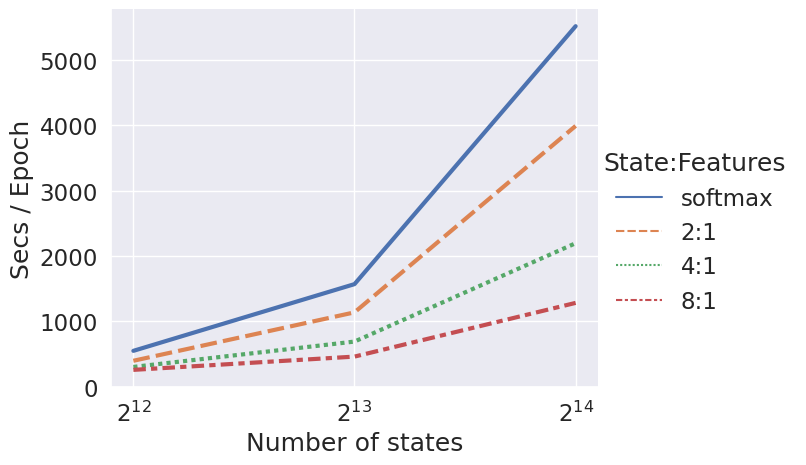
\includegraphics[width=0.48\textwidth]{imgs/hmm/lhmm-states-features-speed.png}
  \vspace*{-0.8cm}
  \caption{\label{fig:speed}
  Speed comparison between softmax HMM and LHMM. 
  %All models converge in 15 epochs.
  }
%\vspace{-0.1cm}
\end{figure}

\vspace{-0.2cm}
\subsection{Comparison to VL-HMM (R1, R5)}
We will also include an explanation of the differences between our LHMM and the VL-HMM (Chiu and Rush, 2020). We note that 
our approach is more general and applies to both HMMs and PCFGs.
Additionally VL-HMM requires hard sparsity structure in the underlying problem. Finally, when this structure does exist,  
%However, thanks to the strict sparsity assumptions, inference in VL-HMMs runs in time independent of the total number of states, whereas inference in LHMMs is linear. 
we believe both approaches can be combined (which we will try in future experiments).

%\textbf{If things work, else delete}
%However, the kernelized inference in LHMMs is orthogonal to the techniques in VL-HMMs. In Figure~\ref{fig:dropout} we showed that state dropout can be applied to LHMMs, and in Figure~\ref{fig:vlhmm} we show that kernelized inference also works with the sparsity constraints behind VL-HMM, allowing us to scale to $2^{16}$ (64k) states.
\vspace{-0.2cm}
\section{Specific Responses}
%\textbf{R1} -Scaling of structured models: The VL-HMM (Chiu and Rush, 2020) demonstrated that bigger HMMs are better, and we validate their observations in Figure~\ref{fig:ppl}. Given this trend holds for both neural and structured models, we believe it will persist.\\
\textbf{R1} -Scaling states: Figure~\ref{fig:ppl} shows improvements with size greatly increased over the original results. \\
%-Small parameter count regularization: Neural network parameterizations allow us to have both large state sizes and regularize with small parameter counts.\\
-Bi-LSTM-CRFs: This approach also applies to CRFs, enabling more efficient marginalization in large label spaces. \\
-LM with PCFG: PCFG is a generative model of a sentence, under which we can compute the likelihood using the inside algorithm.\\
%Perplexity is a function of the likelihood of the text, which can be computed with the inside algorithm.
%-Practicality: Our method applies to graphical models which offer better interpretability than many of their sibling models as a result of model constraints. We hope to eventually prove their practicality by showing that we can achieve strong performance with these constraints, and improving the cost of inference is a necessary step towards that goal. \\
-Practicality: Graphical models provide an alternative  probabilistic view on generative modeling. While the 
aim is to match to performance of NNs, there are also advantages to these models such as interpretability and control. \\
-BERT LM Baseline: This was a mistake, we will remove it.\\
-Clarity of tables/figures: We will fix this in the next version.\\
%-SPEN: Thanks for the reference! \\%We note that exact inference is intractable in SPENs, and we focus on improving the cost of inference in tractable models.\\
\textbf{R2} -More data: We believe more data will help. Our efficient approach also enables using larger datasets.\\
%We believe more data should improve the models greatly. 
-Sample quality: Lower PPLs usually means better samples under the same model class. We will include example samples in the appendix. \\
%\textbf{R3} -Related Work: While our goal was to demonstrate the efficacy of kernelized inference on two widely-used graphical models of increasing complexity, HMMs and PCFGs, the technique should generalize to more interesting models. As such, we are thankful for the reference to one such model! 
%\textbf{R3} -Related work: Thanks for the reference. Our kernelization applies to the feature functions in the segmental hypergraph model, however kernelized inference only reduces complexity if there are at least 1st order interactions. The segmental hypergraph model does not model interactions between neighbouring mention labels. We will compare to this work and elaborate these points in our next version.\\
\textbf{R3} -Related work: Thanks for the reference. Our kernelization applies to the feature functions in the segmental hypergraph model, and would allow the model to include first-order interactions between the mention types of neighbouring words while maintaining the linear runtime. We will elaborate this in our next version.\\
-Comparison to pytorch-struct: The algorithm used for inference in pytorch-struct is logarithmic in the length of the sequence, but cubic in the number of states.
Pytorch-struct is impractical with a large number of states, and with even just 512 states we found our approach to be 600 times faster with 256 features. %(code: \url{https://bit.ly/embedSP}).
\\
\textbf{R5} -Training time: We found both the HMM and LHMM converged at the same number of epochs (15) but LHMM is 2-4x faster for each epoch while achieving similar performance. We will include the learning curves in the appendix.
\end{document}
